\PassOptionsToPackage{english}{babel}
\documentclass{article}

% if you need to pass options to natbib, use, e.g.:
% \PassOptionsToPackage{numbers, compress}{natbib}
% before loading nips_2018

% ready for submission
%\usepackage{nips_2018}

% to compile a preprint version, e.g., for submission to arXiv, add
% add the [preprint] option:
% \usepackage[preprint]{nips_2018}

% to compile a camera-ready version, add the [final] option, e.g.:
\usepackage[final]{nips_2018}

% to avoid loading the natbib package, add option nonatbib:
% \usepackage[nonatbib]{nips_2018}

\usepackage[utf8]{inputenc} % allow utf-8 input
\usepackage[T1]{fontenc}    % use 8-bit T1 fonts
\usepackage{hyperref}       % hyperlinks
\usepackage{url}            % simple URL typesetting
\usepackage{booktabs}       % professional-quality tables
\usepackage{amsfonts}       % blackboard math symbols
\usepackage{nicefrac}       % compact symbols for 1/2, etc.
\usepackage{microtype}      % microtypography
\usepackage{amssymb, amsmath, bm}
\usepackage{color}
\usepackage{float}
\usepackage{graphicx}
\usepackage{graphics}


\newcommand{\ppi}{\bm{\pi}}

\newcommand{\normD}{\mathcal{N}}
\newcommand{\mrm}{\mathrm}
\newcommand{\mbf}{\mathbf}
\newcommand{\mcal}{\mathcal}

\newcommand{\e}{\varepsilon}
\newcommand{\up}{\mathrm}
\def\dbar{\mathrm{\mathchar'26\mkern-12mu d}}
\newcommand{\wave}{\scriptsize{\sim}}
\newcommand{\bb}{\mathbb}
\newcommand{\mbb}{\mathbb}
\newcommand{\imp}[1]{\textit{#1}}
\newcommand{\bs}{\boldsymbol}
\newcommand{\mbs}{\boldsymbol}

\newcommand{\ud}{\mathrm{d}}
\newcommand{\mx}{\mrm x}
\newcommand{\mw}{\mrm w}
\newcommand{\md}{\mrm d}
\newcommand{\mB}{\mrm B}
\newcommand{\mW}{\mrm W}

\newcommand{\TT}{\mbf T}
\newcommand{\UU}{\mbf U}
\newcommand{\VV}{\mbf V}
\newcommand{\XX}{\mbf X}
\newcommand{\ZZ}{\mbf Z}
\newcommand{\WW}{\mbf W}
\newcommand{\RR}{\mbf R}
\newcommand{\MM}{\mbf M}
\newcommand{\KK}{\mbf K}
\newcommand{\II}{\mbf I}
\newcommand{\CC}{\mbf C}


\newcommand{\kk}{\mbf k}
\newcommand{\ww}{\mbf w}
\newcommand{\mm}{\mbf m}
\newcommand{\ttt}{\mbf t}
\newcommand{\bbb}{\mbf b}
\newcommand{\uu}{\mbf u}
\newcommand{\vv}{\mbf v}
\newcommand{\xx}{\mbf x}
\newcommand{\yy}{\mbf y}
\newcommand{\zz}{\mbf z}
\newcommand{\bmu}{\bm{\mu}}
\newcommand{\bphi}{\bm{\phi}}
\newcommand{\bmz}{\bm{0}}

\newcommand{\Exp}{\mathbb{E}}
\newcommand{\rev}{^{-1}}
\newcommand{\calD}{\mcal D}
\newcommand{\data}{\mcal D}
\newcommand{\cat}{\mcal C}
\newcommand{\trans}{^{\mrm T}}
\newcommand{\tit}{\textit}

\newcommand{\subsub}{\subsubsection*}

\title{Reports on PRML Reading Talk}

\author{
  Siyu Wang\\
  Department of Computer Science\\
  Tsinghua University\\
  \texttt{thuwangsy@gmail.com} \\
}

\begin{document}

\maketitle

\section{Introduction to ML, Probability Basics}
\emph{PRML chap.1,2; MLAPP chap.1,2}

The key purpose of machine learning is to extract good \textbf{features} and \textbf{patterns} from \textbf{data}. To realize this purpose, we mainly use function fitting as the tool to solve this problem. In this section we will focus on a polynomial fitting problem, solving it from different angles and considering differences and relations among them. 

But we must keep in mind that, function fitting is only a mathematical tool, not our purpose.

Consider the following problem: given some observed points:
\begin{center}
$D=\{(x_1,t_1),(x_2,t_2), \cdots, (x_N,x_N)\}$
\end{center}
in which, $t = \sin(2\pi x)+\normD(0, \sigma^2)$. Then we want to find a polynomial function
\begin{equation}\label{eq1.1}
    t = y(x,\bf{w})= w_0+w_1x+w_2x^2+...+x_M x^M \tag{1.1}
\end{equation}
to fit these points, so when given new values of $x$, we can predict the corresponding $t$.

\subsection*{From function fitting angle}
We want to optimize the unknown parameter $\mrm{w}$ in equation.\ref{eq1.1} by minimize the \emph{error function}
\begin{equation}\label{eq1.2}
    E(\mrm w) = \frac12\sum_{n=1}^N\{y(x_n, \mrm w)-t_n\}^2.\tag{1.2}
\end{equation}
So we can set the error function's derivative with respect to $\textbf{w}$ to zero and easily get the optimal parameter $\mbf{w}^*$. 

To reduce the over-fitting problem, we may make a little change about the error function by adding a regularization item:
\begin{equation}\label{eq1.3}
    E(\mrm w) = \frac12\sum_{n=1}^N\{y(x_n, \mrm w)-t_n\}^2 + \frac{\lambda}{2}\|\mrm w\|^2. \tag{1.3}
\end{equation}

\subsection*{From probabilistic angle}
Here, we shall assume that, given the value of $x$, the corresponding value of $t$ has a Gaussian distribution with a mean equal to the value $y(x,\mrm{w})$ and a fixed variance $\beta$. So we have 
\begin{equation}
    p(t|x, \mrm w, \beta) = \normD(y(x, \mrm w), \beta^{-1}) \tag{1.4}
\end{equation}

\subsubsection*{MLE: maximum likelihood estimation}
Given $N$ input value $\mbf{x} = (x_1,\cdots, x_N)^T$ and their corresponding target value $\mbf t= (t_1, \cdots, t_N)^T$, we have the likelihood function with the form as 
\begin{equation}
    p(\mbf t|\mbf x, \mrm w, \beta) = \prod_{n=1}^N\normD(t_n|y(x_n,\mrm w),\beta^{-1}). \tag{1.5}
\end{equation}
It's convenient to maximize the logarithm of the likelihood function
\begin{equation}
    \ln p(\mbf t|\mbf x, \mrm w, \beta) = -\frac{\beta}{2}\sum_{n=1}^N\{y(x_n,\mrm w)-t_n\}^2+\frac N2\ln\beta-\frac N2\ln(2\pi). \tag{1.6}
\end{equation}
So when determining $\mbf w$, maximizing likelihood function is equal to minimizing the error function in equation.\ref{eq1.2}. And we obtain
\begin{gather}
    \frac1{\beta_{ML}} = \frac1N\sum_{n=1}^N\{y(x_n,\mrm w_{ML})-t_n\}^2. \tag{1.7}
\end{gather}
So we get a probability distribution of $t$ when given a new value of $x$
\begin{equation}
    p(t|x,\mrm w_{ML},\beta_{ML}) = \normD(t|y(x,\mrm w_{ML},\beta_{ML}) \tag{1.8}
\end{equation}

\subsubsection*{MAP: maximum a posteriori estimation}
Now we take a step towards a more Bayesian approach and introduce a prior distribution over the polynomial coefficient $\mrm w$ and for simplicity, consider a Gaussian distribution of the form 
\begin{equation}
    p(\mrm w|\alpha) = \normD(\mrm w|0,\alpha^{-1}\mrm I) = (\frac\alpha{2\pi})^{(M+1)/2}\exp\{-\frac\alpha2\|w\|^2\} \tag{1.9}
\end{equation}
where $\alpha$ is the precision of the distribution and $M+1$ is the total number of elements in the vector $\mbf w$. Using Bayes' theorem, we can get the posterior distribution for $\mbf w$, which is proportional to the product of the prior distribution and the likelihood function 
\begin{equation}
    p(\mrm w| \mbf x, \mbf t,\alpha, \beta) \propto p(\mbf t|\mrm w, \mbf x, \beta)p(\mrm w|\alpha).  \tag{1.10}
\end{equation}
And finally we find that the maximum of the posterior is given by the minimum of 
\begin{equation}
    \frac\beta2\sum_{n=1}^N\{y(x_n,\mrm w) -t_n\}^2+\frac\alpha2\mrm w^T\mrm w. \tag{1.11}
\end{equation}
Thus we see that maximizing the posterior distribution is equivalent to minimizing the regularized sum-of-square error function in the form (\ref{eq1.3})

\subsection*{Inference and decision}
Here, we come to a classification problem and we have three different approaches to doing inference and decision.
\begin{enumerate}
    \item First solve $p(\mrm{x}|\mathcal C_k)$ as well as $p(\mathcal C_k$ for each class individually, then figure out $p(\mathcal C_k|\mrm x) = \frac{p(\mathrm x|\mathcal C_k)p(\mathcal C_k)}{p(\mrm x)}$ and $p(\mrm x)$ can be gotten from $p(\mrm x) = \sum_kp(\mrm x|\mathcal C_k)p(\mathcal C_k)$. This is equivalent to model the joint distribution $p(\mrm x, \mathcal C_k)$
  \item Determine posterior class probabilities $p(\mathcal C_k|\mrm x)$  and then use decision theory.  \emph{discriminative model}.
  \item Find $f(\mathrm x)$ which maps $\mrm{x}$ directly to a class label.
\end{enumerate}
The first approach is too time-consuming and demanding, while the last one is simplest but not so robust as approach.2 because we can see a lot of information from the posterior probabilities.

\subsection*{For others}
Other than the main ideas and problems discussed above, there are still some other small items here: \emph{Gaussian probability distribution, exponential family, students' t distribution, conjugate prior, } and so on. For more details about these, we can refer to the original book. 

\section{Statistics, Information Theory Basics}
\emph{MLAPP Chap.5,6}
\subsection*{Bayesian Statistics}
Bayes' theorem: 
\begin{equation}
    p(\theta|D)=\frac{p(D|\theta)p(\theta)}{p(D)}
\end{equation}
Priors are assumptions about values of parameters and we can choose an appropriate prior from many different types: \emph{conjugate prior, uninformative prior, robust prior, Jeffreys prior}. 
\subsubsection*{Jeffreys prior}
Given a fixed likelihood $p(\mrm x|\phi)$ where $\mrm x$ represents the data, $\phi$ represents parameters. Then we define Fisher information as the form:
\begin{equation}
    I_{\phi}(\phi)=-\mrm E_{\mrm X\sim p(\mrm x|\phi)}[(\frac{\mrm d\log p(\mrm X|\phi)}{\mrm d\phi})^2]
\end{equation}
and Jeffreys prior is 
\begin{equation}
    p(\phi)\propto(I_{\phi}(\phi))^{1/2}
\end{equation}
An important property of Jeffreys prior is that if we assume $\theta=h(\phi)$, then the prior of $\theta$ is also Jeffreys prior:
\begin{equation}
    p(\theta)\propto (I_{\theta}(\theta))^{1/2}
\end{equation}

And we need to notice that the mixtures of conjugate priors is still a conjugate prior.

\subsubsection*{Hierarchical Bayes}
We can change a 1-level model with the form as:
\begin{equation}
    \theta \rightarrow D
\end{equation}
into a 2-level one by adding a parameter over the prior of $\theta$, then we have
\begin{equation}
    \eta\rightarrow\theta\rightarrow D
\end{equation}
If we apply maximum likelihood respectively to these two models, we can obtain
\begin{gather}
    \mrm{1-level model: }\theta^*=\arg\max_{\theta}p(D|\theta) \\
    \mrm{2-level model: }\eta^*=\arg\max_\eta p(D|\eta)=\arg\max_{\eta}[\int p(D|\theta)p(\theta|\eta)\mrm d\theta]
\end{gather}.
The maximum likelihood for 2-level model is also called \textbf{Empirical Bayes}.
\subsubsection*{Bayesian decision theory}

\subsection*{Frequentist Statistics}
In this part, we see inference from another angle, avoiding treating parameters like random variables, avoiding the use of priors and starting from sampling distribution. 

Given a distribution $p(x|\theta^*)$ where $\theta$ is fixed and we have data $D=(x_1, x_2, \dots, x_n)$ where $x_i\sim p(x|\theta^*)$ and are i.i.d. We want to obtain an estimator $\hat{\theta}=\delta(D)$, which is a function of data to estimate the true parameters $\theta$. 

\section{Linear models(1)}
\emph{MLAPP Chap.7; PRML Chap.3}

In this section, we mainly want to solve the regression problem using a linear model from MLE angle and MAP angle. 
\textbf{Problem setting:} Consider outputs is a linear combination of the inputs 
\begin{equation}
    y(\mbf x) = \mbf w^T\mbf x+\epsilon = \sum_{j=1}^{d}w_jx_j+\epsilon.
\end{equation}
And we can rewrite the model in a probabilistic form:
\begin{equation}
    p(y|\mbf x, \theta) = \normD(y|\mu(\mbf x),\sigma^2(\mbf x)) = \normD(y|\mbf w^T\mbf x, \sigma^2(\mbf x))
\end{equation}
To extend this model linear model, we introduce basis functions, and now the model is 
\begin{equation}
    p(y|\mbf x,\theta) = \normD(y|\mbf w^T\phi(\mbf x),\sigma^2(\mbf x))
\end{equation}
where $\phi$ is a set of functions and $\phi(\mbf x) = (\phi_1(\mbf x), \dots, \phi_M\mbf x)$. And in most cases we assume that $\sigma^2(\mbf x) = \sigma^2$
\subsection*{Maximum Likelihood Estimator}
In this view, we want to find a set of parameters $\theta$ so that likelihood is maximized:
\begin{equation}
    \hat{\theta}=\arg\max_{\theta}\log p(\mathcal D|\theta). 
\end{equation}
And we usually consider the inputs and outputs are i.i.d, so we can obtain
\begin{equation}
    L(\theta) = \log p(\mcal D|\theta)=\log p(\mbf y|\mbf x, \theta) =\sum_{i=1}^{D}\log p(y_i|\mbf x_i,\theta).
\end{equation}
Then we replace $p(y_i|\mbf x_i, \theta)$ by Gaussian distribution, set the derivative with respect to $\mbf w$ to zero and we can obtain
\begin{equation}
    \hat{\mbf w}_{\mrm{MLE}} = (\mbf X^T\mbf X)^{-1}\mbf X^T\mbf y.
\end{equation}
Ans we can understand this method from geometry view. 

There is usually a serious over-fitting problem in MLE so we introduce a regularization item in the object function:
\begin{equation}
    J(\mbf w) = \frac{1}{N}\sum_{i=1}^{N}(y_i-\mbf w^T \mbf x_i)^2+\lambda\|\mbf w\|^2,
\end{equation}
and 
\begin{equation}
    \hat{\mbf w}_{\mrm{ridge}} = (\lambda \mrm I_d +\mbf X^T\mbf X)^{-1}\mbf X^T\mbf y.
\end{equation}

\subsection*{Maximum A Posterior -- Bayesian Linear Regression}
Using Bayes' theorem, we obtain
\begin{equation}
    p(\theta|\mcal D) = \frac{p(\mcal D|\theta)p(\theta)}{p(\mcal D)} \propto p(\mcal D|\theta)p(\theta)
\end{equation}
The conjugate prior corresponding to Gaussian likelihood is still Gaussian, so we assume the prior of $\mbf w$ has a Gaussian form:
\begin{equation}
    p(\mbf w) = \normD (\mbf w|\mbf w_0,\mbf V_0).
\end{equation}
So 
\begin{equation}
    p(\mbf w|\mbf X,\mbf y, \sigma^2)\propto \normD(\mbf w|\mbf w_0,\mbf V_0)\normD(\mbf y|\mbf X,\mbf w,\sigma^2\mbf I_N) = \normD(\mbf w|\mbf w_N,\mbf V_N)
\end{equation}
And if we choose $\mbf V_0=\alpha^{-1}\mbf I$ and $\alpha\rightarrow 0$, we will see $\hat{\mbf w}_{\mrm{MLE}} = \mbf w_N$

\subsubsection*{Bayesian Model Selection}
\begin{equation}
    \mrm{Bayesian factor}:=\frac{p(\mcal D|\mcal M_i)}{p(\mcal D|\mcal M_j)}
\end{equation}
A model $\mcal M_i$ is controlled by a set of parameters $\mbf w$, and 
\begin{equation}
    p(\mcal D|\mcal M_i) = \int p(\mcal D|\mbf w,\mcal M_i)p(\mbf w|\mcal M_i)\mrm d\mbf w.
\end{equation}

\section{Linear models(2)}
\emph{MLAPP Chap.8; PRML Chap.4}

\subsubsection*{Logistic Regression}
Using Bayes Theorem we have 
\begin{equation}
    p(C_1|\mrm x) = \frac{p(\mrm x|C_1)p(C_1)}{p(\mrm x)} = \frac{p(\mrm x|C_1)p(C_1)}{p(\mrm x|C_1)p(C_1)+p(\mrm x|C_2)p(C_2)}=\sigma(a)
\end{equation}
where $a =\log\frac{p(\mrm x|C_2)p(C_2)}{p(\mrm x|C_1)p(C_1)}$.

Suppose $p(\mrm x|C_k)$ is  Gaussian, then we can obtain $a = \mrm w^T\mrm x+\mrm w_0$ and this is very simple to compute $p(C_1|\mrm x)$.

\textbf{Maximum Conditional Likelihood Estimator}.\newline
\begin{equation}
    \hat{\mrm w} = \arg\max_{\mrm x}\prod_{i=1}^{N}p(y_i|\mrm x_i,\mrm w).
\end{equation}
Take the logarithm form to be likelihood function and we have 
\begin{equation}
    L(\mrm w) = -\log\prod_{i=1}^{N}p(y_i|\mrm x_i,\mrm w)=-\sum_{i=1}^{N}\log(p(y_i|\mrm x_i,\mrm w))
\end{equation}
Which is not solvable analytically, so we have no closed-form solution and we need some descent algorithms to minimize $L(\mrm w)$.
\textbf{Gradient descent}
In each iteration, we update the parameter by taking a step backwards the direction which the gradient points to
\begin{equation}
    \mrm w^{(\tau+1)} = \mrm w^{\tau}-\eta \nabla_{\mrm w}L(\mrm w)
\end{equation}

\subsubsection*{Bayesian Logistic Regression}
Estimate the posterior of parameters $\mrm w$ rather than just a point estimation.

\textbf{Generative model}: learn a model of the \textbf{joint probability}, $p(x, y)$, of the inputs $x$ and the label $y$, and make their predictions by using Bayes rules to calculate $p(ylx)$, and then picking the most likely label $y$.\newline
\textbf{Discriminative model}: learn the posterior $p(ylx)$ directly, or learn a direct map from inputs $x$ to the class labels.

\section{Kernels}
\emph{MLAPP Chap.14; PRML Chap.6,7}

A big difference between this chapter and previous ones is that here, the training data points or s subset of them are kept during the prediction phase rather than are discarded.  and predictions for new inputs are based purely on the learned parameter vector $\ww$.

\emph{radial basis functions:} depend only on the magnitude of the distance between the arguments so that 
\begin{equation}
    k(\xx,\xx')=k(\|\xx-\xx'\|).
\end{equation}
Gram matrix is a matrix with kernel values as its elements. And a Gram matrix is Mercer when it is non-negative definite. 

\subsection{Construction of kernels}
One approach is to choose a feature space mapping $\phi(\xx)$ and then use it to find the corresponding kernel. 
\begin{equation}
    k(\xx,\xx')=\phi(\xx)\trans\phi(\xx') = \sum_{i=1}^{M}\phi_i(\xx)\phi_i(\xx').
\end{equation}
But, an alternative approach is to construct kernel functions directly, at the same time, we should ensure it is valid.  A necessary and sufficient condition for a function $k(\xx, \xx') $ to be a valid kernel is that the Gram matrix $\mbf  K$ whose elements are given by $k(\xx_n,\xx_m)$, should be positive semi-definite for all possible choices of the set $\{\xx_n\}$.

There are a series of techniques to construct valid kernels out of simpler kernels. A commonly used kernel takes the from:
\begin{equation}
    k(\xx,\xx') = \exp(-\|\xx-\xx'\|^2/2\sigma^2)
\end{equation}
which is called Gaussian kernel. And another powerful approach to constructing kernels starts from a probabilistic generative model:
\begin{equation}
    k(\xx,\xx') = p(\xx)p(\xx').
\end{equation}

\subsection{Radial Basis Function Networks}
Expressing $f(\xx)$ as a linear combination of radial basis functions, one centred on every data point 
\begin{equation}
    f(\xx) = \sum_{n=1}^N w_nh(\|\xx-\xx_n\|)
\end{equation}
and we can use least square s to find $\{w_n\}$. 
\subsubsection*{Nadaraya-Waatson model}
Assume a Parzen density estimator to model the joint distribution $p(\xx, t) $ so that :
\begin{equation}
p(\xx,t) = \frac1N\sum_{n=1}^{N}f(\xx-\xx_n,t-t_n)
\end{equation}
$f(\cdot)$ is the component density function. And finally we can obtain :
\begin{equation}
k(\xx,\xx_n) = \frac{g(\xx-\xx_n)}{\sum_mg(\xx-\xx_m)}
\end{equation}
where $g(\xx) = \int_{-\infty}^{\infty}f(\xx,t)\mathrm dt$
with a property that gives more weight to the data points $\xx_n$ that are close to $\xx$.

\subsection{Sparse kernel}
Here we shall look at kernel-based algorithms that have sparse solutions, so that predictions for new inputs depend only on the kernel function evaluated at a subset of the training data points. 

\textit{SVM} is a decision machine and so does not provide posterior probabilities. It has a property that the  determination of the model parameters corresponds to a convex optimization problem, and so any local solution is also a global optimum.
\subsubsection*{Maximum Margin Classifiers}
\emph{Margin} is defined as the smallest distance between the decision boundary and any of  the samples. The idea of SVM is to choose a boundary that maximize margin. Here, when the data set if not linearly seperable in the original space, we can project them into another feature space using basis functions $\phi(\cdot)$ to make them linearly separable. 

\section{Graphical Models}
\emph{MLAPP Chap.10,19; PRML Chap 8.1-8.3}

We shall find it highly advantageous to augment the analysis using diagrammatic representations of probability distributions, called \textit{probabilistic graphical models}. These offer several useful properties:
\begin{enumerate}
    \item They provide a simple way to visualize the structure of a probabilistic model and can be used to design and motivate new models.
    \item Insights into the properties of the model, including conditional independence properties, can be obtained by inspection of the graph.
    \item Complex computations, required to perform inference and learning in sophisticated models, can be expressed in terms of graphical manipulations, in which underlying mathematical expressions are carried along implicitly.
\end{enumerate}
We have random variables as \emph{nodes} and probabilistic relationships between variable as \emph{links}. 

Then we focus on \emph{Bayesian Networks}. First we can decomposite a joint probability distribution in the form 
\begin{equation}
    p(a, b, c) = p(c|a, b)p(b|a)p(a).
\end{equation}
Then we can extend to $K$ variables:
\begin{equation}
    p(x_1,\dots, x_K) = p(x_K|x_1,\dots,x_{K-1})\dots p(x_2|x_1)p(x_1). 
\end{equation}
And the corresponding directed graph is called \emph{fully connected} because there is a link between every pair of nodes. And we can write it in a simple form
\begin{equation}
    p(\xx) = \prod_{k=1}^Kp(x_k|\mrm{pa}_k)
\end{equation}
where $\mrm{pa}_k = \mrm{pa}(k)$ denotes the set of parents of node $x_k$. 

The directed graphs that we are considering are subject to an important restriction namely that there must be no \textit{directed cycles}, in other words there are no closed paths within the graph such that we can move from node to node along links following the direction of the arrows and end up back at the starting node. Such graphs are also called \textit{directed acyclic graphs}, or \textit{DAGs}. This is equivalent to the statement that there exists an ordering of the nodes such that there are no links that go from any node to any lower numbered node.

There are three basic structures in Bayesian networks: \emph{head-to-head, head-to-tail, tail-to-tail}, and the example can be seen in \ref{fig6.1}
\begin{figure}[H]
    \centering
    \includegraphics[width=\textwidth]{./figures/fig6_1.png}
    \caption{Basic structures of Bayesian networks}
    \label{fig6.1}
\end{figure}

Then, we can do d-separation on a DAG. Suppose $\mcal C$ is a set of random variables, $a$ and $b$ are two variables that are not in $\mcal C$. We call $\mcal C$ 'd-separate' $a$ and $b$ iff for any route from $a$ to $b$:
\begin{itemize}
    \item if any node $v$ is on the route is head-to-head or head-to-tail, $v\in \mcal C$.
    \item if any node $v$ on the route is tail-to-tail, $v\notin \mcal C$ and $\mrm{de}(v)\notin \mcal C$ where $\mrm{de}(v)$ denotes the set of descendants of node $v$. 
\end{itemize}

\section{Latent Variable Model, Clustering and EM}
\emph{MLAPP Chap.11,25; PRML Chap.9}

In this section, We use mixture models to cluster data, as well as build more complex probability distributions. Therefore we begin our discussion of mixture distributions by considering the problem of finding clusters in a set of data points. Then we introduce the latent variable view of mixture distributions in which the discrete variables can be interpreted as defining assignments of data points to specific component of the mixture. Finally we discuss EM in some generality.
\subsection{K-means}
Suppose we have input data set $\{\mrm x_1,\cdots, \mrm x_N\}$ consisting of $N$ observations of a random $D-$dimensional Euclidean variable $\mrm x$. Our goal is to partition the data set into some number $K$ of clusters.  Firstly we consider a fixed value of $K$. We can formalize this notion by first introducing a set of $D-$dimensional vectors $\mu_k$, where $k=1,\cdots,K$, in which $\mu_k$ is a prototype associated with the $k^{th}$ cluster. For each data point $\mrm x_n$, we introduce a corresponding set of binary indicator variables $r_{nk} \in \{0,1\}$, describing which cluster $\mrm x_n$ is assigned to. We can then define an objective function
\begin{equation}
J = \sum_{n=1}^{N}\sum_{k=1}^{K}r_{nk}\|\mrm x_n-\mu_k\|^2.
\end{equation}

Firstly we choose some initial values for the $\mu_k$. Then in the first phase we minimize $J$ with respect to the $r_{nk}$, keeping the $\mu_k$ fixed. In the second phase we minimize $J$ with respect to the $\mu_k$, keeping $r_{nk}$ fixed. This two-stage optimization is then repeated until convergence. And we obtain
\begin{gather}\label{}
  r_{nk}=\{\begin{matrix}
                 1 & \mrm{if }k=\mrm{arg min_j}\|\mrm x_n-\mu_j\|^2 \\
                 0 & \mrm{otherwise}.
               \end{matrix} \\
  \mu_k = \frac{\sum_nr_{nk}\mrm x_n}{\sum_nr_{nk}}
\end{gather}
A direct implementation of the $K-$means algorithm as discussed here cna be slow because in each E step it is necessary to compute the Euclidean distance between every prototype vector and every data point. Various schemes have been proposed for speeding up this algorithm.

\subsection{Mixture of Gaussian}
The Gaussian mixture distribution can be written as linear superposition of Gaussians  in the form
\begin{equation}\label{}
  p(\mbf x) = \sum_{k=1}^{K}\pi_k\normD(\mbf x|\mu_k,\Sigma_k).
\end{equation}
Then we can introduce a $K-$dimensional binary random variable $\mbf z$ having a 1-of-$K$ representation in which a particular element $z_k$ is equal to 1 and all other elements are equal to 0. So $z_k \in \{0,1\}$, $\sum_{k}z_k=1$, and $p(z_k=1)=\pi_k$. So
\begin{equation}\label{}
  p(\mrm z) = \prod_{k=1}^{K}\pi_k^{z_k}.
\end{equation}
So the marginal distribution of $\mrm x$ is then obtained:
\begin{equation}\label{}
  p(\mrm x) = \sum_{\mrm z}p(\mrm z)p(\mrm x|\mrm z) = \sum_{k=1}^{K}\pi_k\normD(\mrm x|\mu_k,\Sigma_k)
\end{equation}
And we can gain the conditional probability of $\mrm z$ given $\mrm x$ using Bayes' theorem
\begin{equation}\label{eq3.3.0}
  \gamma(z_k) \equiv p(z_k=1|\mrm x)=\frac{p(z_k=1)p(\mrm x|z_k=1)}{\sum_{j=1}^{K}p(z_j=1)p(\mrm x|z_j=1)} =  \frac{\pi_k\normD(\mrm x|\mu_k, \Sigma_k)}{\sum_{j=1}^{K}\pi_j\normD(\mrm x|\mu_j,\Sigma_j)}.
\end{equation}
Suppose we have a data set of observations $\{\mrm x_1, \cdots, \mrm x_N\}$, and we wish to model this data using a mixture of Gaussians. Denote this data set as an $N\times D$ matrix $\mrm X$ in which the $n^{th}$ row is given by $\mrm x_n^T$, latent variables as an $N\times K$ matrix $\mrm Z$ with rows $\mrm z_n^T$. Assume i.i.d observations, we can obtain ;pg likelihood function in the form:
\begin{equation}\label{}
  \ln p(\mrm X|\pi, \mu, \Sigma) = \sum_{n=1}^{N}\ln\{\sum_{k=1}^{K}\pi_k\normD(\mrm x_n|\mu_k, \Sigma_k)\}.
\end{equation}

\subsection{EM algorithm for Gaussian mixtures}
We can not formulate a closed-form solution for maximum log likelihood, so we may use EM algorithm to solve the problem :
\begin{enumerate}
  \item Initialize the means $\mu_k$, covariances $\Sigma_k$ and mixing coefficients $\pi_k$, and evaluate the initial value of the log likelihood.
  \item \textbf{E step.} Evaluate the responsibilities using the current parameter values.
  \item \textbf{M step.} Re-estimate the parameters using the current responsibilities.
  \item Evaluate the log likelihood
  \begin{equation}\label{}
    \ln p(\mrm X|\mu,\Sigma,\pi)=\sum_{n=1}^{N}\ln \{\sum_{k=1}^{K}\pi_k\normD(\mrm x_n|\mu_k,\Sigma_k)\}
  \end{equation}
\end{enumerate}

\section{Continuous Latent Variables}
\emph{MLAPP Chap.12,13; PRML Chap.12}

This section is lectured by myself.

\section{Exact Inference}
\emph{MLAPP Chap.20; PRML Chap.8.4}
% \subsection{Exact Inference}
\subsection{Inference on a Chain}
Consider the graph shown in figure\ref{fig9.1}. The joint distribution for this graph takes the form
\begin{figure}[H]
    \centering
    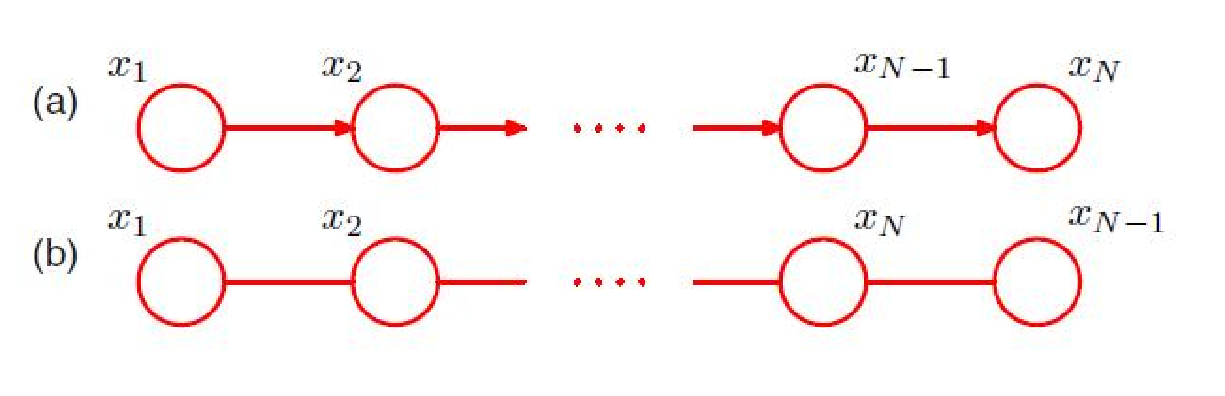
\includegraphics[width=\textwidth]{./figures/GM3.eps}
    \caption{Chain Model}
    \label{fig9.1}
\end{figure}
\begin{equation}\label{eq8.16}
  p(\bf x) = \frac{1}{Z}\psi_{1,2}(x_1,x_2)\psi_{2,3}(x_2,x_3)...\psi_{N-1,N}(x_{N-1},x_N).
\end{equation}
If we want to get marginal distribution $p(x_n)$ for a specific node, we should sum the joint distribution over all variables except $x_n$, so that
\begin{equation}\label{eq8.17}
  p(x_n) = \sum_{x_1}...\sum_{x_{n-1}}\sum_{x_{n+1}}...\sum_{x_N}p(\bf x)
\end{equation}
But this way will cost so much computational resources, so we want to find another simpler way:
\begin{align}\label{eq8.18}
  p(x_n) =  & \frac{1}{Z}[\sum_{x_{n-1}}\psi_{n-1,n}(x_{n-1},x_n)\dots[\sum_{x_2}\psi_{2,3}(x_2,x_3)[\sum_{x_1}\psi_{1,2}(x_1,x_2)]]\dots] \\
   & [\sum_{x_{n+1}}\psi_{n,n+1}(x_n,x_{n+1})\dots[\sum_{x_N}]\psi_{N-1,N}(x_{N-1},x_{N})]\dots]  \\
   = & \frac{1}{Z}\mu_{\alpha}(x_n)\mu_{\beta}(x_n)
\end{align}
As shown in figure\ref{fig9.2}, we can see message passed in the chain and we can compute $\mu_{\alpha}(x_i)$ and $\mu_{\beta}(x_i)$ recursively for any $i=1, 2, \dots, N$.
\begin{equation}\label{eq8.19}
  \mu_{\alpha}(x_n) = \sum_{x_{n-1}}\psi_{n-1,n}(x_{n-1},x_n)\mu_{\alpha}(x_{n-1}).
\end{equation}
and
\begin{equation}\label{eq8.20}
  \mu_{\alpha}(x_2) = \sum_{x_1}\psi_{1,2}(x_1,x_2).
\end{equation}
Similar for $\mu_{\beta}(x_n)$
\begin{figure}[H]
  \centering
  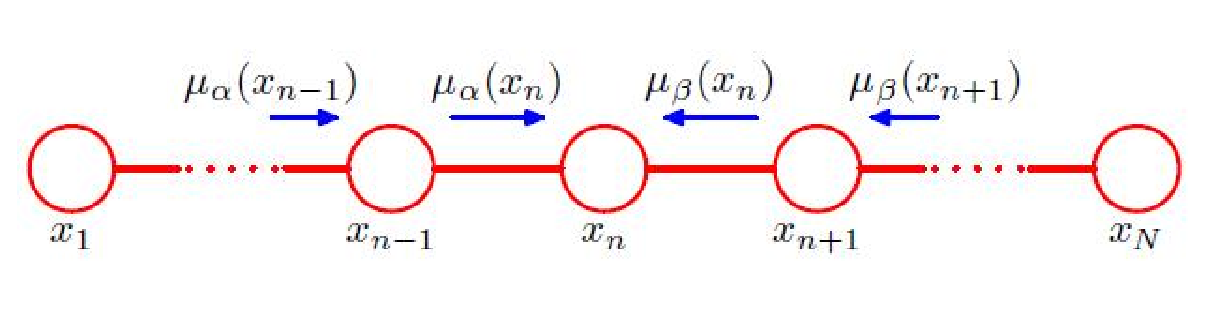
\includegraphics[width=\textwidth]{./figures/GM4.eps}
  \label{fig9.2}
\end{figure}
\subsection{Inference on a Tree: sum-product algorithm}
\subsubsection*{factor graphs}
In a factor graph, there is a node (depicted as usual by \textbf{a circle}) for every variable
in the distribution, as was the case for directed and undirected graphs. There are also
additional nodes (depicted by \textbf{small squares}) for each factor fs(xs) in the joint distribution.\newline
For example,
\begin{equation}\label{eq8.21}
  p(\bf{x}) = f_a(x_1,x_2)f_b(x_1,x_2)f_c(x_2,x_3)f_d(x_3)
\end{equation}
can be expressed by the factor graph shown in figure\ref{GM5}
\begin{figure}
  \centering
  \includegraphics[width=0.5\textwidth]{./figures/GM5.jpg}
  \caption{Example of a factor graph}\label{GM5}
\end{figure}
Factor graphs are said to be bipartite because they consist of two distinct kinds
of nodes, and all links go between nodes of opposite type.
\subsubsection*{sum-product algorithm}
We shall now make use of the factor graph framework to derive a powerful class
of efficient, exact inference algorithms that are applicable to tree-structured graphs.
Here we shall focus on the problem of evaluating local marginals over nodes or
subsets of nodes, which will lead us to the sum-product algorithm.\newline
Our goal is to exploit the structure of
the graph to achieve two things: (i) to obtain an efficient, exact inference algorithm
for finding marginals; (ii) in situations where several marginals are required to allow
computations to be shared efficiently.
\textbf{finding the marginal $p(x)$ for a particular variable node $x$}\newline
$$p(\bf x) = \prod_{s\in ne(x)}F_s(x,X_s)   $$
$$p(x) = \prod_{s\in ne(x)}[\sum_{X_s}F_s(x,X_s)] = \prod_{s\in ne(x)}\mu_{f_s\rightarrow x}(x) $$
$$F_s(x,X_s) =  f_s(x,x_1,...x_M)G_1(x,X_{s1})...G_M(x,X_{sM})$$
$$\mu_{x_m\rightarrow f_s}(x_m) \equiv \sum_{X_{sm}}G_m(x_m,X_{sm})$$
We have therefore introduced two distinct kinds of message, those that go from factor
nodes to variable nodes denoted $\mu_{f\rightarrow x}(x)$, and those that go from variable nodes to
factor nodes denoted $\mu_{x\rightarrow f}(x).$
\textbf{Illustration: example}
\textbf{max-sum algorithm}
Two other common tasks are to find a setting of the variables that has the largest probability
and to find the value of that probability. We therefore seek an efficient algorithm for finding the value of x that maximizes
the joint distribution p(x) and that will allow us to obtain the value of the
joint distribution at its maximum.
\subsection{Inference on a Graph}
Here we will discuss graphs with loops. Our method is \textbf{Loopy belief propagation}
One simple approach to approximate inference in graphs with
loops, which builds directly on the previous discussion of exact inference in trees.
The idea is simply to apply the sum-product algorithm even though there is no guarantee
that it will yield good results. For some graphs, the algorithm will converge, whereas for others it will not. \newline
We will say that a (variable or factor) node a has a message pending on its link to a node b if node a has received any
message on any of its other links since the last time it send a message to b.

\section{Variational Inference}
\emph{MLAPP Chap.21,22; PRML Chap.10}

So far we have several inferences: 
\begin{itemize}
    \item Compute the likelihood of observed data.
    \item Compute the marginal distribution.
    \item Compute the conditional probability.
\end{itemize}
And we have several methods to do exact inference:
\begin{itemize}
    \item Brute force
    \item Elimination
    \item Message passing
\end{itemize}
Also there are several approximation inference techniques such as sampling method, MCMC and variational algorithms.

In variational inference, we want to approximate the target distribution $p$ by a 'simpler' distribution $q$, and we will turn the inference problem into a constrained optimization problem. Then we introduce KL-divergence as our optimization objective. 

\subsection{KL divergence}
Suppose we have a set of observed variables $\xx$ and latent variables $\zz$. We want to infer 
\begin{equation}
    p(\zz|\xx) = \frac{p(\xx,\zz)}{p(\xx)}.
\end{equation}
When it's hard to compute $p(\zz|\xx)$, we may find an approximation $q(\zz)$. And KL divergence between these two distributions are defined as follow:
\begin{equation}
    \mrm{KL}(q(\zz)||p(\zz)) = \int_{\zz}q(\zz)\log \frac{q(\zz)}{p(\zz)}\mrm d\zz = \Exp_{q(\zz)}[\log \frac{q(\zz)}{p(\zz)}].
\end{equation}
So our goal is to find a distribution $q(\zz)$ to minimize the KL divergence:
\begin{equation}\label{eq10.1}
    q^*(\zz) = \arg\max_{q(\zz)\in \mcal Q}\mrm{KL}(q(\zz)||p(\zz|\xx)).
\end{equation}
This objective is however intractable :
\begin{align}
    \mrm{KL}(q(\zz)||p(\zz|\xx)) & = \int q(\zz)\log\frac{q(\zz)}{p(\zz|\xx)}\mrm d\zz \\
    & =\Exp_{q(\zz)}[\log q(\zz)]-\Exp_{q(\zz)}[\log p(\zz,\xx)]+\log p(\xx) \\
    & = -\mathbb H(q)- \Exp_{q(\zz)}[\log p(\zz,\xx)] +\log p(\xx).
\end{align}

\subsection{Evidence Lower Bound}
We define 
\begin{equation}
    \mrm{ELBO}(q) = -\mrm{KL}(q(\zz)||p(\zz|\xx)) +\log p(\xx) =  \mathbb H(q) + \Exp_{q(\zz)}[\log p(\zz,\xx)].
\end{equation}
Then the minimization problem formulated in \ref{eq10.1} can be transformed into 
\begin{equation}
    q^*(\zz) = \arg\max_{q(\zz)}\mrm{ELBO}(q).
\end{equation}
And we notice that when the KL divergence is 0, $\mrm{ELBO}(q)$ is maximized. 

Also we can obtain another view of ELBO by dissecting the variational objective. We can show that it mirrors the usual balance between likelihood and the prior:
\begin{align}
    \mrm{ELBO} (q) & = \Exp_{q(\zz)}[\log p(\zz,\xx)]-\Exp_{q(\zz)}[\log q(\zz)] \\
     & = \Exp_{q(\zz)}[\log p(\zz)] + \Exp_{q(\zz)}[\log p(\xx|\zz)]-\Exp_{q(\zz)}[\log q(\zz)] \\
     & = \Exp_{q(\zz)}[\log p(\xx|\zz)] + \Exp_{q(\zz)}[\log \frac{p(\zz)}{q(\zz)}] \\
     & = \Exp_{q(\zz)}[\log p(\xx|\zz)] - \mrm{KL}(q(\zz)||p(\zz))
\end{align}
where $\Exp_{q(\zz)}[\log p(\xx|\zz)]$ denotes the expected log-likelihood of the data conditional on latent variables so that it encourages the (variational) densities that place their mass on configurations of the
latent variables that explain the observed data, i.e. increases the likelihood. The second term $ \mrm{KL}(q(\zz)||p(\zz))$ denotes that it encourages the density to be closer to prior in order to minimize divergence. 

\subsection{Mean field methods}
Mean field method is a way to restrict $q(\zz)$ to an "easier" family. We assume that $q$ distribution can be factorized as follows:
\begin{equation}
    q(\zz) = \prod_{i=1}^Mq_i(\zz_i)
\end{equation}
where $\zz$ is partitioned into disjoint groups $\zz_i$.   Then, we obtain coordinate ascent algorithm to optimize ELBO. 

\section{Monte Carlo}
\emph{MLAPP Chap.23,24; PRML Chap.11}
\subsection{Monte Carlo Inference}
\subsubsection*{Standard distribution}
\subsub{Reject sampling}
\subsub{Importance sampling}
\subsection{Markov Chain Monte Carlo}
\subsub{Markov chain}
\begin{equation}
    p(\xx_{1:\tau}) = p(\xx_1)p(\xx_2|\xx_1)\dots p(\xx_\tau|\xx_{\tau-1})
\end{equation}
Stationary distribution $\bm{\pi}$:
\begin{equation}
    \ppi = \ppi\mbf A
\end{equation}
We say that a Markov chain $\mbf A$ is time reversible if there exists a distribution 
\textcolor{red}{xxx}

The basic idea in Metroplis-Hasting is that at each step, we propose to move from current state $\xx$ to a new state $\xx'$ with probability $q(\xx'|\xx)$ 

\section{Sequential Data}
\emph{MLAPP Chap.17,18; PRML Chap.13}

\section{Gaussian Process}
\emph{MLAPP Chap.15}

Here we want to approximate a function $y= f(\xx)$ be a linear function in the form 
\begin{equation}
    y(\xx) = \ww\trans\phi(\xx)
\end{equation}
where $\phi(\xx)$ is a vector composed by $M$ fixed basis functions $\phi_j(\xx),\ j=1,2,\dots,M$. Then we assume the prior distribution over $\ww$:
\begin{equation}
    p(\ww) = \normD(\ww|\bmz, \alpha\rev\mbf I).
\end{equation}
Then given training data set $\{\xx_1, \dots, \xx_N\}$ with targets $\{t_1,\dots, t_N\}$ . We denote $\yy = (y_1,\dots, y_2)\trans,\ y_n=y(\xx_n).$, then 
\begin{equation}
    \yy =  \Phi\ww
\end{equation}
where $\phi$ is a matrix with elements $\Phi_{nk}=\phi_k(\xx_n)$. So we have $\Exp[\yy]=\bmz,\ \mrm{cov}[\yy\yy\trans] = \frac{1}{\alpha}\Phi\Phi\trans=\KK$, where $K_{nm}=k(\xx_n,\xx_m)=\frac{1}{\alpha}\phi\trans(\xx_n)\phi(\xx_m)$

\subsection{Gaussian process for regression}
For regression problem, we assume our sampling target points $t_n$ is obtained by adding a noise $\epsilon$ to the true target number $y_n$:
\begin{equation}
    t_n=y_n+\epsilon.
\end{equation}
So 
\begin{gather}
    p(t_n|y_n)=\normD(t_n|y_n, \beta\rev) \\
    p(\ttt|\yy) = \normD(\ttt|\yy,\beta\rev\mbf I)
\end{gather}
Then we can obtain the marginal distribution of $\ttt$:
\begin{equation}
    p(\ttt) = \int p(\ttt|\yy)p(\yy)\ud\yy=\normD(\ttt|\bmz, \CC)
\end{equation}
where 
\begin{equation}\label{eq13.1}
    \CC_{nm}=k(\xx_n,\xx_m)+\beta\rev\delta_{nm}.
\end{equation}
Although we obtain this result via $k(\xx_n,\xx_m) = \frac1\alpha\phi\trans(\xx_n)\phi(\xx_m)$, now we can discard this to make our model more flexible. Usually we choose the \emph{kerel function} $k(\cdot,\cdot))$ as 
\begin{equation}
    k(\xx_n,\xx_m)=\theta_0\exp\{-\frac{\theta_1}{2}\|\xx_n-\xx_m\|^2\}+\theta_2+\theta_3\xx_n\trans\xx_m.
\end{equation}

Then we want to find the conditional distribution $p(t_{N+1}|\ttt)$. First,
\begin{equation}
    p(\ttt_{N+1}) = \normD(\ttt_{N+1}|\bmz, \CC_{N+1})
\end{equation}
where $\CC_{N+1}$ is defined by \ref{eq13.1} while $N$ is substituted with $N+1$, and we can partition it in the form
\begin{equation}
    \CC_{N+1}=\left(\begin{array}{cc}
         \CC_N & \kk  \\
         \kk\trans & c 
    \end{array}\right)
\end{equation}
where $\CC_N$ is just defined by \ref{eq13.1}, $\kk$ has elements $k(\xx_n,\xx_{N+1})$ and the scalar $c = k(\xx_{N+1},\xx_{N+1})+\beta\rev$.
Using knowledge in Gaussian probability, we can obtain the conditional distribution $p(t_{N+1}|\ttt_N)$ is still Gaussian with mean and variance given by 
\begin{gather}\label{eq13.2}
    \Exp[t_{N+1}] = m(\xx_{N+1})=\kk\trans\CC_N\ttt, \\
    \mrm{var}[t_{N+1}] = \sigma^2(\xx_{N+1})=c-\kk\trans\CC_N\rev\kk,
\end{gather}
where these functions is relied on $\xx_{N+1}$ through $\kk$ because $\kk$ is defined by $k(\xx_n,\xx_{N+1}$.

Note that the only restriction on the kernel function is that the covariance matrix given by  \ref{eq13.1} is positive definite. And if kernel matrix is positive semidefinite, the requirement will certainly be satisfied.  

Note that the mean given by \ref{eq13.2} of the predictive distribution can be written, as a function of $\xx_{N+1}$, in the form
\begin{equation}
    m(\xx_{N+1})=\sum_{n=1}^Na_nk(\xx_n, \xx_{N+1})
\end{equation}
where $a_n$ is the $n^{\mrm{th}}$ component of $\CC_N\rev\ttt$. Thus, the kernel function depends only on the distance $\|\xx_n-\xx_m\|$, then we obtain an expansion in \emph{radial basis functions}.

\subsection{Gaussian process for classification}
Define a Gaussian process on $a(\xx)$ then transform it using a logistic sigmoid $y=\sigma(a)$, so we obtain a non-Gaussian stochastic process over $y(\xx)$ where $y\in\{0,1\}$. Then the probability distribution over the target variable $t$ is then given by the Bernoulli distribution 
\begin{equation}
    p(t|a)=\sigma(a)^t(1-\sigma(a))^{1-t}.
\end{equation}

As usual, we denote $\xx_1,\dots,\xx_N$, $\ttt$, then we consider a single test point $\xx_{N+1}$. Our goal is to determine the predictive distribution $p(t_{N+1}|\ttt)$, where we have left the conditioning on the input variables implicit. To do this we introduce a Gaussian process 
prior over the vector $\mbf a_{N+1}$, which has components $a(\xx_1), \dots, a(\xx_{N+1})$. 
\begin{equation}
    p(\mbf a_{N+1}) = \normD(\mbf a_{N+1}|\bmz,\CC_{N+1}).
\end{equation}
Unlike the regression case, the covariance matrix no longer includes a noise term because we assume that all of the training data points are correctly labelled. However, for numerical reasons it is convenient to introduce a noise-like term governed by a parameter $\nu$ that ensures that the covariance matrix is positive definite. Thus 
\begin{equation}
    \CC(\xx_n,\xx_m) = k(\xx_n,\xx_m)+\nu\delta_{nm}
\end{equation}
where $k(\xx_n,\xx_m)$ is any positive semidefinite kernel function. And we assume the kernel function is governed by parameters $\bm{\theta}$. 

For two-class problem, it is sufficient to predict $p(t_{N+1}=1|\ttt_N)$:
\begin{equation}
    p(t_{N+1}=1|\ttt_N) = \int p(t_{N+1}=1|a_{N+1})p(a_{N+1}|\ttt_N)\ud a_{N+1}
\end{equation}
where $p(t_{N+1}=1|a_{N+1})=\sigma(a_{N+1})$. The integral is analytically intractable so we want to use a Gaussian distribution to approximate the logistic function. There are generally three approaches:
\begin{itemize}
    \item \emph{variational inference}. make use of the local variational bound on the logistic sigmoid. 
    \item \emph{expectation propagation}.
    \item Laplace approximation. 
\end{itemize}

\section{Neural Network}
\emph{MLAPP Chap.16, PRML Chap.5}
In this section, our focus is on neural networks as efficient models for statistical pattern recognition.
\subsection{Feed-forward Network Functions}
The linear models for regression and classification, respectively, are based on linear combinations of fixed nonlinear basis functions $\phi_j(\mathrm x)$ and take the form
\begin{equation}\label{eq2.4.1}
  y(\mathrm x,\mathrm w) = f(\sum_{j=1}^Mw_j\phi_j(\mathrm x))
\end{equation}
where $f(\cdot)$ is a nonlinear activation function in the case of classification and is the identity in the case of regression. Our goal is to extend this model by making the basis function $\phi_j(\mathrm x)$ depend on parameters and then allow these parameters to be adjusted, along with the coefficients $\{w_j\}$, during training.

For the first layer,
\begin{gather}\label{}
a_j=\sum_{j=1}^Dw_{ji}^{(1)}x_i+w_{j0}^{(1)} \\
z_j=h(a_j)
\end{gather}
This quantities correspond to the outputs of the basis functions in eq\ref{eq2.4.1} that, in the context of neural networks, are called \textit{hidden units}. The activation functions $h(\cdot)$  are generally chosen to be sigmoidal function or the 'tanh'. Following eq\ref{eq2.4.1} these values are again linearly combined to give \textit{output unit activations}
\begin{equation}\label{}
  a_k=\sum_{j=1}^{M}w_{kj}^{(2)}z_j+w_{k0}^{(2)}
\end{equation}
where $k=1,\dots,K$ and $K$ is the total number of outputs. Finally, the output unit activations are transformed using an appropriate activation function to give a set of network output $y_k$. For standard regression problems, the activation function is the identity so that $y_k=a_k$. Similarly, for multiple binary classification problems, $y_k =\sigma(a_k)$. And for multiclass problems, a softmax function is used.

Combining these various stages to give the overall network function that, for sigmoidal output unit activation functions, we obtain
\begin{equation}\label{eq2.4.2}
  y_k(\xx,\ww) = \sigma(\sum_{j=1}^{M}w_{kj}^{(2)}h(\sum_{i=1}^{D}w_{ji}^{(1)}x_i+w_{j0}^{(1)})+w_{k0}^{(2)})
\end{equation}
where the set of all weight and bias parameters have been grouped together into a vector $\ww$. The process of evaluating \ref{eq2.4.2} can then be interpreted as a \textit{forward propagation} of information through the network.

One property of feed-forward networks, which will play a role when we consider Bayesian model comparison, is that multiple distinct choices for the weight vector
$\ww$ can all give rise to the same mapping function from inputs to outputs.
\subsection{Network Training}
There is a simple idea to train the parameter: minimize the error function. e.g.
\begin{equation}\label{eq2.4.3}
  E(\ww) = \frac12\sum_{n=1}^N\|\yy(\xx_n,\ww)-\ttt_n\|^2
\end{equation}
However we can provide a more general view of network training by first giving a probabilistic interpretation to the network outputs.

Consider firstly \textbf{regression problem} with a single target variable $t$ and $t$ has a Gaussian distribution with an $\xx$-dependent mean:
\begin{equation}\label{eq2.4.4}
p(t|\xx,\ww)=\normD(t|y(\xx,\ww), \beta\rev).
\end{equation}
For the conditional distribution given by \ref{eq2.4.4}, it is sufficient to take the output unit activation function to be identity. Given a data set of $N$  i.i.d observations $\XX =\{\xx_1,\dots,\xx_N$ along with corresponding target values $\ttt = \{t_1,\dots,t_N\}$, we can construct the corresponding likelihood function
\begin{equation}\label{}
  p(\ttt|\XX,\ww,\beta)=\prod_{n=1}^{N}p(t_n|\xx_n,\ww,\beta).
\end{equation}
Taking the negative logarithm, we obtain the error function
\begin{equation}\label{}
  \frac{\beta}{2}\sum_{n=1}^{N}\{y(\xx_n,\ww)-t_n\}^2-\frac{N}{2}\ln \beta+\frac N2\ln(2\pi).
\end{equation}
Consider first the determination of $\ww$, we want to minimize the error function given by
\begin{equation}\label{}
  E(\ww)=\frac12\sum_{n=1}^{N}\{y(\xx,\ww)-t_n\}^2.
\end{equation}
The value of $\ww$ found by minimizing $E(\ww)$ will be denoted $\ww_{\mrm{ML}}$. Then
\begin{equation}\label{}
  \frac{1}{\beta_{\mrm{ML}}}=\frac1N\sum_{n=1}^{N}\{y(\xx_n,\ww_{\mrm{ML}}-t_n\}^2.
\end{equation}

Then consider the case of \textbf{binary classification problem}. The conditional distribution given inputs is then a Bernoulli distribution of the form
\begin{equation}\label{}
  p(t|\xx,\ww) = y(\xx,\ww)^t\{1-y(\xx,\ww)\}^{1-t}.
\end{equation}
If we consider a training set, then the error function is then a \textit{cross-entropy} error function  of the form
\begin{equation}\label{}
  E(\ww) = \sum_{n=1}^{N}\{t_n\ln y_n+(1-t_n)\ln (1-y_n)\}
\end{equation}

Finally we consider the standard multiclass classification problem in which each input is assigned to one of $K$ mutually exclusive classes, and the networks outputs are interpreted as $y_k(\xx,\ww) = p(t_k=1|\xx)$, leading to the following error function
\begin{equation}\label{}
  E(\ww) = -\sum_{n=1}^{N}\sum_{k=1}^{K}t_{kn}\ln y_k(\xx_n,\ww).
\end{equation}
And the output unit activation function is given by
\begin{equation}\label{}
  y_k(\xx,\ww) = \frac{\exp(a_k(\xx,\ww)}{\sum_j\exp(a_j(\xx_n,\ww))}
\end{equation}
\subsubsection*{Parameter optimization}
Then we turn next to the task of finding a weight vector w which minimizes the chosen function $E(\mathrm w)$. But the error function typically has a highly nonlinear dependence on the weights and bias parameters, and so there will be many points in weight space at which the gradient vanishes.

Because there is clearly no hope of finding an analytical solution to the equation $\nabla E(\ww) = 0$ we resort to iterative numerical procedures.\textbf{The optimization of continuous nonlinear functions is a widely studied problem.} Most techniques involve choosing some initial value $\ww^{(0)}$ for the weight vector and then moving through weight space in a succession of steps of the form
\begin{equation}\label{eq2.4.6}
  \ww^{(\tau+1)} = \ww^{(\tau)}+\delta\ww^{(\tau)}.
\end{equation}
Then gradient information is important here. So we consider a local approximation of the error function based on Taylor expansion.

\subsubsection*{Local quadratic approximation}
Consider the Taylor expansion of $E(\ww)$ around some point $\hat \ww$ in weight space
\begin{equation}\label{eq2.4.5}
  E(\ww) \simeq E(\hat \ww)+(\ww-\hat \ww)\trans \bbb+\frac12(\ww-\hat \ww)\trans\mbf H(\ww-\hat \ww)
\end{equation}
where
\begin{equation}\label{}
  \bbb \equiv \nabla E|_{\ww=\hat\ww}
\end{equation}
and the Hessian matrix $\mbf H =\nabla\nabla E$.

From \ref{eq2.4.5}, we obtain
\begin{equation}\label{}
  \nabla E \simeq  \bbb+\mbf H(\ww-\hat\ww).
\end{equation}

Considering the minimum point $\ww^*$, we have
\begin{equation}\label{}
  E(\ww) = E(\ww^*)+\frac12(\ww-\ww^*)\trans\mbf H(\ww-\ww^*).
\end{equation}
So if $\ww^*$ is a minimum point, the Hessian matrix $\mbf H$ should be \textit{positive definite}, which means all the eigenvalues of $\mbf H$ is positive.
\subsubsection*{Gradient descent optimization}
The simplest approach to using gradient information is to choose the weight update in \ref{eq2.4.6} to comprise a small step in the direction of the negative gradient, so
that
\begin{equation}\label{}
  \ww^{(\tau+1)} =\ww^{(\tau)}-\eta\nabla E(\ww^{(\tau)})
\end{equation}
where $\eta$ is called \tit{learning rate}. Note that the whole data set is used and this technique was once called \tit{batch} method. At each step the weight vector is moved in the direction of the greatest rate of decrease of the error function, and so this approach is known as \tit{gradient descent} or \tit{steepest descent}.

For batch optimization, there are more efficient methods, such as \tit{conjugate gradients} and \tit{quasi-Newton} methods.

Also, there is an online version of gradient descent called \tit{sequential gradient descent or stochastic gradient descent}, make update to the weight vector based on one data point at a time, so that
\begin{equation}\label{}
  \ww^{(\tau+1)}=\ww^{(\tau)} -\eta\nabla E_n(\ww^{(\tau)}).
\end{equation}

\subsection{Error Backpropagation}
\textbf{Goal}: find an efficient technique for evaluating  the gradient of an error function $E(\mathrm w)$ for a feed-forward neural network.

\textbf{Algorithm}:
\begin{enumerate}
  \item Apply an input vector xn to the network and forward propagate through the network to find the activations of all the hidden and output units.
  \item Evaluate the $\delta k$ for all the output units using.
  \item Backpropagate the $\delta$’s using to obtain $\delta j$ for each hidden unit in the network.
  \item Evaluate the required derivatives.
\end{enumerate}

\subsection{Regularization in Neural Networks}
To avoid over-fitting, we can add a regularizer to the error function:
\begin{equation}\label{}
  \tilde{E}(\ww) = E(\ww)+\frac{\lambda}{2}\ww\trans\ww.
\end{equation}
This regularizer can be interpreted as the negative logarithm of a zero-mean Gaussian prior distribution over the weight vector $\ww$.

There are also many other ways to avoid over-fitting:
\begin{itemize}
  \item Early stopping
  \item Invariance
  \item Tangent propagation
  \item Training with transformed data
\end{itemize}
More details can be found in section5.5 in \tit{PRML}.

\section{Deep Learning}
\emph{MLAPP Chap.28}
Given a data set $\mcal D = \{\xx_1,\dots, \xx_N\} \sim p(\xx)$, we want  to find the distribution $p(\xx)$. 


\section{Combining Models}
\emph{PRML Chap.14}
\end{document}